%Master File:lectures.tex

\lesson{When Machine Learning Works}
\vspace{-1cm}
\begin{center}
\noindent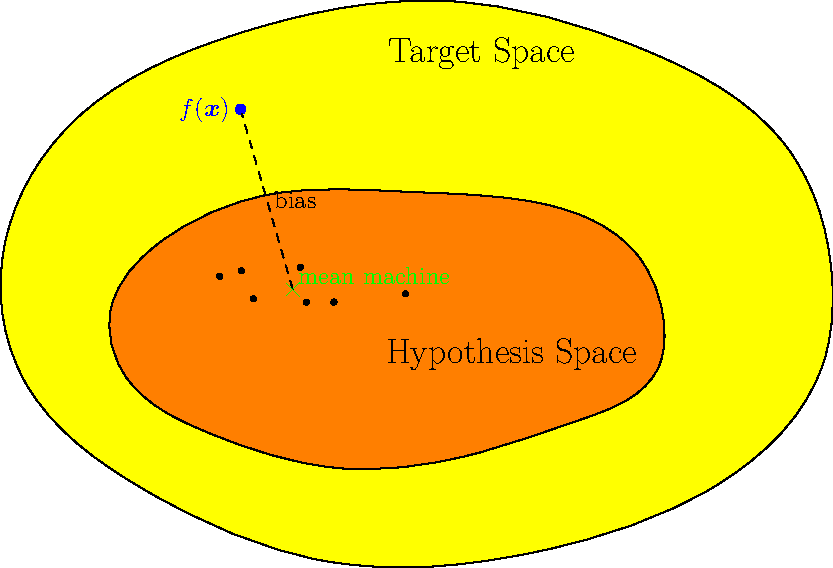
\includegraphics[height=100mm]{approxEstim-17}
\end{center}
\keywords{When ML Works, Bias Variance}
%%%%%%%%%%%%%%%%%%%%%%% Next Slide %%%%%%%%%%%%%%%%%%%%%%%
\renewcommand{\Outline}{%
\begin{slide}
\section[1]{Outline}

\begin{minipage}{12cm}\raggedright
  \begin{enumerate}\squeeze
    \outlineitem{What Makes a Good Learning Machine?}{why}
    \outlineitem{Bias-Variance Dilemma}{dilemma}
  \end{enumerate}
\end{minipage}\hfill
\begin{minipage}{10cm}
  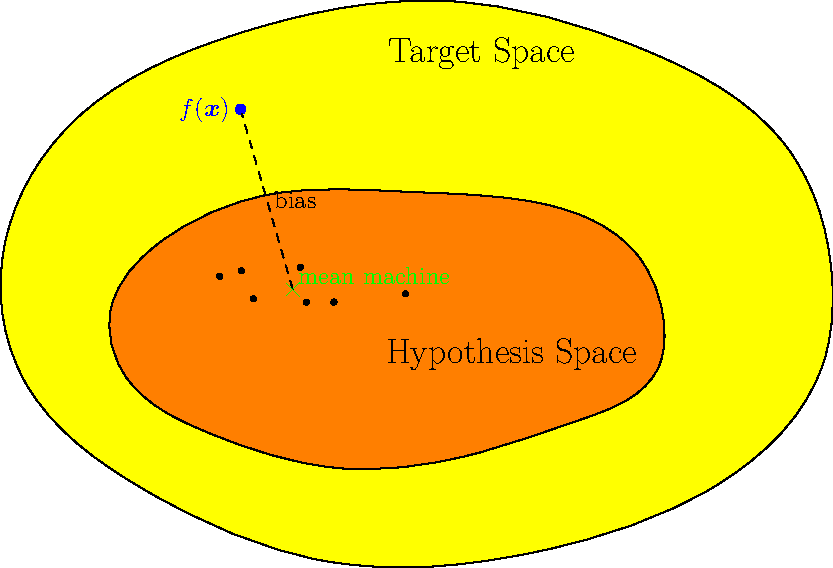
\includegraphics[width=10cm]{approxEstim-17}
\end{minipage}
\end{slide}
\addtocounter{outlineitem}{1}
}

\setcounter{outlineitem}{1}

%%%%%%%%%%%%%%%%%%%%%%% Next Slide %%%%%%%%%%%%%%%%%%%%%%%
\Outline % Why ML works
\toptarget{firstoutline}
%%%%%%%%%%%%%%%%%%%%%%% Next Slide %%%%%%%%%%%%%%%%%%%%%%%


\begin{slide}
\section{What Makes a Good Learning Machine?}

\begin{PauseHighLight}
  \begin{itemize}
  \item We want to understand why some machine learning techniques
    work well and other don't\pause
  \item To understand why these works we need to understand what makes a
    good learning machine\pause
  \item For this we have to get conceptual and think about
    \emph{generalisation} performance\pause
    \begin{quote}\it
      \textbf{generalisation}: how well do we do on unseen data as
      opposed to the training data\pause
    \end{quote}
  \end{itemize}
\end{PauseHighLight}

\end{slide}

%%%%%%%%%%%%%%%%%%%%%%% Next Slide %%%%%%%%%%%%%%%%%%%%%%%

\begin{slide}
\section{What Makes Machine Learning Hard?}

\begin{PauseHighLight}
  \begin{itemize}
  \item Typically work in high dimensions (i.e. have many
    features)\pause
  \item The problem can be over-constrained (i.e. we have conflicting
    data to deal with)\pause---solve by minimising an error function\pauseb
  \item The problem can be under-constrained (i.e. there are many
    possible solutions that are consistent with the data)\pause---need to
    choose a plausible solution\pauseb
  \item Typically in machine learning the data will be over-constrained
    in some dimensions and under-constrained in others\pause
  \item We can't visualise the data to know what is going
    on\pause
  \end{itemize}
\end{PauseHighLight}

\end{slide}

%%%%%%%%%%%%%%%%%%%%%%% Next Slide %%%%%%%%%%%%%%%%%%%%%%%

\begin{slide}
\section{Least Squared Errors}

\begin{PauseHighLight}
  \begin{itemize}
  \item Suppose we want to learn some output $y$ for a feature vector $\bm{x}$\pause
  \item We construct a learning machine that makes a prediction
    $\hat{f}(\bm{x}|\bm{\theta})$\pause
  \item We typically choose the machine to  minimise a \textit{training loss}
    \begin{align*}
      L_T(\mathcal{D}) = \sum_{(\bm{x},y)\in\mathcal{D}} \left(
      \hat{f}(\bm{x}|\bm{\theta}) - y \right)^2 \pause
      = \sum_{i=1}^m \left(
      \hat{f}(\bm{x}_i) - y_i \right)^2
    \end{align*}
    where $\mathcal{D} = \{(\bm{x}_i, y_i)\}_{i=1}^m$ is a set of
    size $m$, sampled a probability distribution $\mu(\bm{x},y)$\pauseb
  \item We call this machine $\hat{f}(\bm{x}\vert \bm{\theta}_\mathcal{D})$\pauseb
  \end{itemize}
\end{PauseHighLight}

\end{slide}

%%%%%%%%%%%%%%%%%%%%%%% Next Slide %%%%%%%%%%%%%%%%%%%%%%%

\begin{slide}
\section{Generalisation Error}

\begin{PauseHighLight}
  \begin{itemize}
  \item We want to minimise the \textit{generalisation loss} which in
    this case is
    
    \begin{rightImage}{sampleSpace}
      \begin{align*}
        L_G(\mathcal{D}) = \sum_{(\bm{x},y)\in\mathcal{Z}} \mu(\bm{x},y)\,
        \left(\hat{f}(\bm{x}\vert \bm{\theta}_\mathcal{D}) - y
        \right)^2\pause 
      \end{align*}
    \end{rightImage}

    (we can estimate this if we have some labelled examples
    $(\bm{x}_i,y_i)$ which we have not trained on)\pause
  \item We want to minimise $L_G(\mathcal{D})$ but in practice we are
    minimising $L_T(\mathcal{D})$, \textit{what could possibly go wrong?}\pause
  \end{itemize}
\end{PauseHighLight}

\end{slide}

%%%%%%%%%%%%%%%%%%%%%%% Next Slide %%%%%%%%%%%%%%%%%%%%%%%

\begin{slide}
\section[-2]{Too Simple or Too Complex?}

\pb
\hypertarget{regression}{}

\begin{itemize}
\item Fit $\hat{f}(x|\bm{\theta}_\mathcal{D})$ to data\pauseh
  \begin{center}
    \multipdf{curveFitting}\pause
  \end{center}
\end{itemize}

\end{slide}


%%%%%%%%%%%%%%%%%%%%%%% Next Slide %%%%%%%%%%%%%%%%%%%%%%%

\begin{slide}
\section[-1]{Measuring Generalisation Error for Regression}

\begin{PauseHighLight}

\begin{itemize}
\item Consider the regression example.  The root mean squared error
  is
  \begin{center}
    \noindent\includegraphics[height=120mm]{rmsErrors}
  \end{center}\pause
\end{itemize}

\end{PauseHighLight}
\end{slide}

%%%%%%%%%%%%%%%%%%%%%%% Next Slide %%%%%%%%%%%%%%%%%%%%%%%
\Outline % Bias-Variance Dilemma
%%%%%%%%%%%%%%%%%%%%%%% Next Slide %%%%%%%%%%%%%%%%%%%%%%%

\begin{slide}
\section{Expected Generalisation Performance}

\begin{PauseHighLight}
  \begin{itemize}
  \item Our generalisation performance will depend on our training set,
    $\mathcal{D}$\pause
  \item To reason about generalisation we can ask what is the
    \textit{expected generalisation loss}, when we average over
    all different data sets of size $m$ drawn independently from
    $\mu(\bm{x},y)$\pause
  \item For each data set, $\mathcal{D}$, we would learn a different
    approximator $\hat{f}(\bm{x}\vert \bm{\theta}_\mathcal{D})$\pause
  \item Note that in practice we only get one data set.  We might be
    lucky and do better than the expected generalisation or we might be
    unlucky and do worse\pause
  \end{itemize}
\end{PauseHighLight}

\end{slide}

%%%%%%%%%%%%%%%%%%%%%%% Next Slide %%%%%%%%%%%%%%%%%%%%%%%

\begin{slide}
\section[-2]{Approximation and Estimation Errors}
\pb\pause\pauselevel{=1}
\begin{center}
  \multipdf[width=0.9\linewidth]{approxEstim}\pause
\end{center}

\end{slide}

%%%%%%%%%%%%%%%%%%%%%%% Next Slide %%%%%%%%%%%%%%%%%%%%%%%

\begin{slide}
\section{Mean Machine}

\begin{PauseHighLight}
  \begin{itemize}
  \item To help understand generalisation we can consider the mean
    prediction with respect to machines trained with all data sets of
    size $m$
    \begin{align*}
      \hat{f}_m(\bm{x}) = \av[\mathcal{D}]{ \hat{f}\left(\bm{x} |
      \bm{\theta}_{\mathcal{D}}\right)} \pause
    \end{align*}
  \item We can define the \emph{bias} to be generalisation performance
    of the mean machine
    \begin{align*}
      B = \sum_{\bm{x}\in\mathcal{X}} \mu(\bm{x},y) \left( \hat{f}_m(\bm{x})
      - y \right)^2\pause
    \end{align*}
  \end{itemize}
\end{PauseHighLight}

\end{slide}



%%%%%%%%%%%%%%%%%%%%%%% Next Slide %%%%%%%%%%%%%%%%%%%%%%%
\whitepage
\begin{slide}
\section[-1]{Regression Example $n=1$}
\toptarget{regress}

\pb\pause\pauselevel{=1}
\begin{center}
  \includegraphics[width=18cm]{bv11}\pause
  \llap{\includegraphics[width=18cm]{bv12}}\pause
  \llap{\includegraphics[width=18cm]{bv13}}\pause
  \llap{\includegraphics[width=18cm]{bv14}}\pause
\end{center}

\end{slide}



%%%%%%%%%%%%%%%%%%%%%%% Next Slide %%%%%%%%%%%%%%%%%%%%%%%
\whitepage
\begin{slide}
\section[-1]{Regression Example $n=5$}

\pb\pause\pauselevel{=1}
\begin{center}
  \includegraphics[width=18cm]{bv21}\pause
  \llap{\includegraphics[width=18cm]{bv22}}\pause
  \llap{\includegraphics[width=18cm]{bv23}}\pause
  \llap{\toplink{regresscont}{\includegraphics[width=18cm]{bv24}}}\pause
\end{center}
\end{slide}

%%%%%%%%%%%%%%%%%%%%%%% Next Slide %%%%%%%%%%%%%%%%%%%%%%%
\renewcommand{\mypl}[1]{\pauselevel{=#1 :}\pause}
\begin{slide}
\section[-2]{Bias and Variance}

\pb
Consider the expected generalisation for data sets of size $|\mathcal{D}|=m$
\begin{align*}
  \bar{L}_G &= \av[\mathcal{D}]{ L_G(\mathcal{D}) } \pause
            = \av[\mathcal{D}]{  \sum_{\bm{x}\in\mathcal{X}} \mu(\bm{x},y)\,
              \left(\hat{f}(\bm{x}\vert \bm{\theta}_{\mathcal{D}}) -
              y \right)^2}\pause
  \\
  &=  \sum_{\bm{x}\in\mathcal{X}} \mu(\bm{x},y)\,
  \av[\mathcal{D}]{ 
  \left(\hat{f}(\bm{x}\vert \bm{\theta}_{\mathcal{D}}) - y \right)^2}\pause
  \\
      &= \sum_{\bm{x}\in\mathcal{X}} \mu(\bm{x},y)\, \av[\mathcal{D}]{
        \left(\mypl{4}\left(\mypl{5}\hat{f}(\bm{x}\vert
        \bm{\theta}_{\mathcal{D}})
        -\hat{f}_m(\bm{x}) \mypl{4}\right)\mypl{5} + \mypl{4}\left(\mypl{5}
        \hat{f}_m(\bm{x}) - y \mypl{4}\right)\mypl{5} \right)^2
        }\mypl{4} \\
            &=  \sum_{\bm{x}\in\mathcal{X}} \mu(\bm{x},y) \Biggl(
              \av[\mathcal{D}]{ 
              \left(\hat{f}(\bm{x}\vert \bm{\theta}_{\mathcal{D}}) -
              \hat{f}_m(\bm{x}) \right)^2 + \left(
              \hat{f}_m(\bm{x}) - y \right)^2 }  \\
            & \hspace{5cm} + 2 \, \av[\mathcal{D}]{
              \left(\hat{f}(\bm{x}\vert \bm{\theta}_{\mathcal{D}}) -
              \hat{f}_m(\bm{x}) \right)\left(
              \hat{f}_m(\bm{x}) - y \right) } \Biggr)\mypl{6}
\end{align*}

\end{slide}
%%%%%%%%%%%%%%%%%%%%%%% Next Slide %%%%%%%%%%%%%%%%%%%%%%%

\begin{slide}
\section{Cross Term}

\begin{PauseHighLight}
  \begin{itemize}
  \item The cross term vanishes
  \begin{align*}
  C &= \av[\mathcal{D}]{ \left(\hat{f}(\bm{x}\vert \bm{\theta}_{\mathcal{D}}) -
              \hat{f}_m(\bm{x}) \right)\left(
              \hat{f}_m(\bm{x}) - y \right) }\pause\\
     &= \left(\av[\mathcal{D}]{\hat{f}(\bm{x}\vert \bm{\theta}_{\mathcal{D}})} -
              \hat{f}_m(\bm{x}) \right)\left(
              \hat{f}_m(\bm{x}) - y \right)\pauseb\\
     &= \left(\hat{f}_m(\bm{x}) -
              \hat{f}_m(\bm{x}) \right)\left(
              \hat{f}_m(\bm{x}) - y \right)\pauseb\\
              &= 0\pauseb
  \end{align*}
  \item Thus
  \begin{align*}
   \bar{L}_G &= \sum_{\bm{x}\in\mathcal{X}} \mu(\bm{x},y)
              \av[\mathcal{D}]{ 
              \left(\hat{f}(\bm{x}\vert \bm{\theta}_{\mathcal{D}}) -
              \hat{f}_m(\bm{x}) \right)^2 + \left(
              \hat{f}_m(\bm{x}) - y \right)^2 }\pauseb
  \end{align*}
  \end{itemize}
\end{PauseHighLight}

\end{slide}



%%%%%%%%%%%%%%%%%%%%%%% Next Slide %%%%%%%%%%%%%%%%%%%%%%%

\begin{slide}
\section[-2]{Bias and Variance}

\begin{PauseHighLight}
  \begin{itemize}
  \item We can write the expected generalisation loss as
    \begin{align*}
      \av[\mathcal{D}]{ L_G(\mathcal{D}) }
      &= \sum_{\bm{x}\in\mathcal{X}} \mu(\bm{x},y)\, 
      \av[\mathcal{D}]{ \left(\hat{f}(\bm{x}\vert \bm{\theta}_{\mathcal{D}}) -
      \hat{f}_m(\bm{x})\right)^2 } \\
        & \quad \quad +
          \sum_{\bm{x}\in\mathcal{X}} \mu(\bm{x},y) \left( \hat{f}_m(\bm{x})
      - y \right)^2 \pause
        = V + B\pause
    \end{align*}
  \item Where $B$ is the bias and $V$ is the variance defined by
    \begin{align*}
      V = \sum_{\bm{x}\in\mathcal{X}} \mu(\bm{x},y)\,
      \av[\mathcal{D}]{ \left(\hat{f}(\bm{x}\vert \bm{\theta}_{\mathcal{D}}) -
      \hat{f}_m(\bm{x})\right)^2 }\pause 
    \end{align*}
  \end{itemize}
\end{PauseHighLight}

\end{slide}

%%%%%%%%%%%%%%%%%%%%%%% Next Slide %%%%%%%%%%%%%%%%%%%%%%%

\begin{slide}
\section{Bias-Variance Dilemma}

\begin{PauseHighLight}
  \begin{itemize}
  \item The bias measure the generalisation performance of the
    \textit{mean machine} and is large if the machine is too simple to
    capture the changes in the function we want to learn\pause
  \item The variance measures the variation in the prediction of the
    machine as we change the data set we train on
    \begin{align*}
      V =  \sum_{\bm{x}\in\mathcal{X}} \mu(\bm{x},y)\,
      \av[\mathcal{D}]{ \left(\hat{f}(\bm{x}\vert \bm{\theta}_{\mathcal{D}})
      - \hat{f}_m(\bm{x})\right)^2 }\pause
    \end{align*}
  \item \toplink{regress}{The variance is usually large if we have a complex machine}\pause
    \toptarget{regresscont}
  \item Striking the right balance is often the key to getting good
    results\pause 
  \end{itemize}
\end{PauseHighLight}

\end{slide}

%%%%%%%%%%%%%%%%%%%%%%% Next Slide %%%%%%%%%%%%%%%%%%%%%%%

\begin{slide}
\section[-1]{Balancing Bias and Variance}

\begin{PauseHighLight}
  \begin{itemize}
  \item We want to choose a learning machine that is complex enough to
    capture the underlying function we are trying to learn, but
    otherwise as simple as possible\pause
  \item There are a number of tricks to achieve this balance\pause
  \item Some require us to preprocess the data to reduce the number of
    inputs\pause
  \item Some machines cleverly adjust their own complexity\pause
  \item This course looks at machines that achieve this balance\pause
  \end{itemize}
\end{PauseHighLight}

\end{slide}

%%%%%%%%%%%%%%%%%%%%%%% Next Slide %%%%%%%%%%%%%%%%%%%%%%%

\begin{slide}
\section[-2]{Lessons}

\begin{PauseHighLight}
  \begin{itemize}
  \item This course is about understanding machine learning techniques that
    work well\pause
  \item Which one to use will depend on the data set\pause
  \item One of the most useful intuitions about what works is the
    bias-variance framework\pause
  \item The bias is high for simple machines that can't capture the
    data\pause
  \item The variance is high for complex machines that are sensitive
    to the training set\pause
  \item Good machines are powerful enough to capture complex data sets,
    but they can control their own capacity (ability to (over-)fit the
    data)\pause
  \end{itemize}
\end{PauseHighLight}

\end{slide}


%%% Local Variables:
%%% TeX-master: "lectures"
%%% End:
